        \subsection{Fourier series}

\begin{frame}{fundamentals}{Fourier series --- introduction}
    youtube --- mechanical analyzer:
    
    \url{http://youtu.be/6dW6VYXp9HM}
\end{frame}
\begin{frame}{fundamentals}{Fourier series --- complex representation 1/2}
    \begin {equation}
        x(t) = \sum\limits_{k=0}^{N} a_k \sin(k\omega_0 t + \Phi_k) \nonumber
    \end {equation}
    \pause
    \begin{itemize}
        \item   trigonometric identity $\sin(a+b) = \sin(a)\cos(b) + \cos(a)\sin(b)$
        \item[$\Rightarrow$]
        \only<2>{
        \begin{equation}
            x(t) = \sum\limits_{k=0}^{N} {a_k \sin(\Phi_k)}\cdot\cos(k\omega_0 t) + {a_k \cos(\Phi_k)}\cdot\sin(k\omega_0 t)\nonumber
        \end{equation}
        }
        \only<3->{
        \begin{equation}
            x(t) = \sum\limits_{k=0}^{N} \underbrace{a_k \sin(\Phi_k)}_{A_k}\cdot\cos(k\omega_0 t) + \underbrace{a_k \cos(\Phi_k)}_{B_k}\cdot\sin(k\omega_0 t)\nonumber
        \end{equation}
        }
    \end{itemize}
\end{frame}
\begin{frame}{fundamentals}{Fourier series --- complex representation 2/2}
    \begin{eqnarray}
        e^{\mathrm{j}\omega t} &=& \cos(\omega t) + \mathrm{j}\sin(\omega t)\nonumber\\
        \mathrm{j} &=& \sqrt{-1}\nonumber
    \end{eqnarray}
    \pause
    \begin{itemize}
        \item   phasor representation in complex plane
    \end{itemize}
    \pause
		\begin{flushright}
			 
\includegraphics[scale=.08]{Graph/question-mark}
		\end{flushright}
    \begin{eqnarray}
        \cos(\omega t) &=& \only<3>{?}\only<4->{\frac{1}{2}\left(e^{\mathrm{j}\omega t} + e^{-\mathrm{j}\omega t}\right)}\nonumber\\
        \sin(\omega t) &=& \only<3>{?}\only<4->{\frac{1}{2\mathrm{j}}\left(e^{\mathrm{j}\omega t} - e^{-\mathrm{j}\omega t}\right)}\nonumber
    \end{eqnarray}
\end{frame}
\begin{frame}{fundamentals}{Fourier series 1/2}
	\begin{itemize}
		\item	any periodic signal $\Rightarrow$ representation in \textbf{Fourier Series}
			\only<1>{
			\begin {equation}
				x(t) = \sum\limits_{k=-\infty}^{\infty} c_k \e^{\mathrm{j}\omega_0 kt} \nonumber
			\end {equation}}
			\only<2>{
			\begin {equation}
				x(t) = \sum\limits_{k=-\infty}^{\infty} c_k \e^{\mathrm{j}\textcolor{gtgold}{\omega_0} kt} \nonumber
			\end {equation}}
			\only<3>{
			\begin {equation}
				x(t) = \sum\limits_{k=-\infty}^{\infty} c_k \textcolor{gtgold}{\e^{\mathrm{j}\omega_0 kt}} \nonumber
			\end {equation}}
			\only<4>{
			\begin {equation}
				x(t) = \sum\limits_{k=-\infty}^{\infty} \textcolor{gtgold}{c_k} \e^{\mathrm{j}\omega_0 kt} \nonumber
			\end {equation}}
			\only<5>{
			\begin {equation}
				x(t) = \sum\limits_{k=-\infty}^{\infty} c_k \e^{\mathrm{j}\omega_0 kt} \nonumber
			\end {equation}}
			\pause
			\begin{itemize}
				\item	$\omega_0 = 2\pi\cdot f_0$
				\pause
				\item	$\e^{\jom_0kt} = \cos(\omega_0kt) + \mathrm{j} \sin(\omega_0kt)$	\nonumber		
			\end{itemize}
	
		\pause
		\item	Fourier series coefficients $c_k$
			\begin {equation}\label{eq:fourier_coeff}
				c_k = \frac{1}{T_0}\int\limits_{-\nicefrac{T_0}{2}}^{\nicefrac{T_0}{2}} x(t) \e^{-\jom_0kt}\, dt \nonumber
			\end {equation}
	\end{itemize}
\end{frame}

\begin{frame}{fundamentals}{Fourier series 2/2}
	reconstruction of periodic signals with a limited number of sinusoidals:
	\begin {equation}
		\hat{x}(t) = \sum\limits_{k=-\mathcal{K}}^{\mathcal{K}} c_k e^{\jom_0kt}
	\end {equation}
	\only<1>{
	\begin{figure}
		\centering
			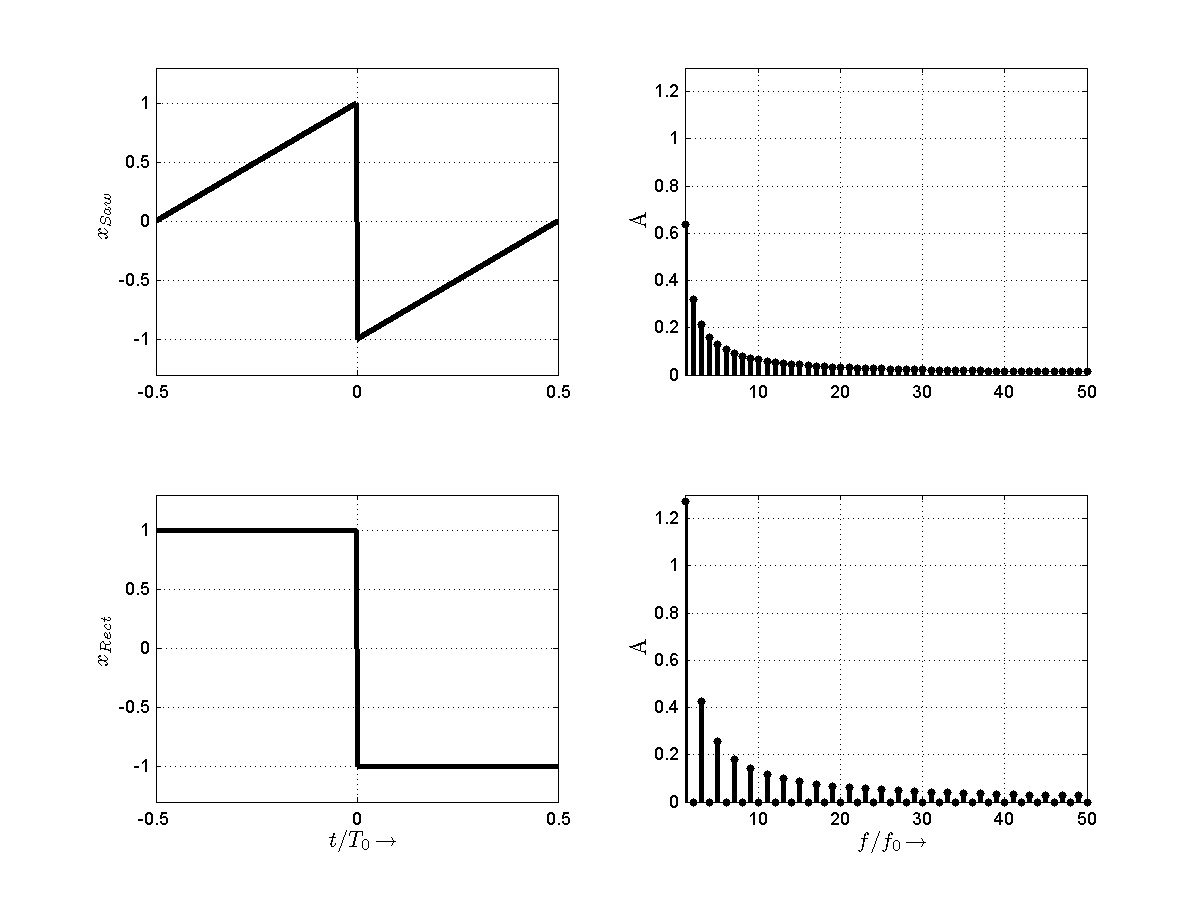
\includegraphics[height=4cm,width=\textwidth]{graph/additivesynthesis-1}
	\end{figure}
	}
	\only<2->{
    \begin{center}
        \animategraphics[scale=.5,autoplay,loop]{10}{graph/FourierSeriesSquare/frame_}{000}{059}        
        \hspace{5mm}\animategraphics[scale=.5,autoplay,loop]{10}{graph/FourierSeriesSaw/frame_}{000}{059}  
    \end{center}
	}
\end{frame}

\begin{frame}{fundamentals}{conjugate complex multiplication}
    \begin{figure}
        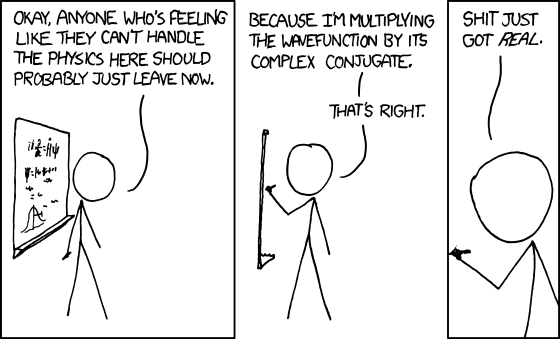
\includegraphics[scale=.45]{graph/xkcd_complex_conjugate}
    \end{figure}
    
    from \url{https://xkcd.com/849}
\end{frame}

\begin{frame}{fundamentals}{Fourier series --- real to complex}
    \vspace{-5mm}
    \begin{footnotesize}
    \begin{eqnarray}
        \cos(\omega t) &=& \frac{1}{2}\left(e^{\jom t} + e^{-\jom t}\right)\nonumber\\
        \sin(\omega t) &=& \frac{1}{2\mathrm{j}}\left(e^{\jom t} - e^{-\jom t}\right)\nonumber
    \end{eqnarray}
    \pause
    \vspace{-2mm}
    \begin{eqnarray}
        x(t) &=& \sum\limits_{k=0}^{\infty} A_k\cos(k\omega t) + B_k\sin(k\omega t)\nonumber\\
        &=& \sum\limits_{k=0}^{\infty} \frac{A_k}{2}\left(e^{\jom kt} + e^{-\jom kt}\right) - \mathrm{j}\frac{B_k}{2}\left(e^{\jom kt} - e^{-\jom kt}\right)\nonumber\\
        &=& \sum\limits_{k=0}^{\infty} \frac{1}{2}\left(A_k-\mathrm{j}B_k\right)e^{\jom kt} +  \frac{1}{2}\left(A_k+\mathrm{j}B_k\right)e^{-\jom kt}\nonumber\\
        &=& \sum\limits_{k=0}^{\infty} \underbrace{\frac{1}{2}\left(A_k-\mathrm{j}B_k\right)}_{c_k}e^{\jom kt} +  \frac{1}{2}\left(A_k+\mathrm{j}B_k\right)e^{-\jom kt}\nonumber
    \end{eqnarray}
    \begin{equation}\nonumber
       \text{with } c_{-k} := c^\ast_k \Rightarrow\;\; x(t) = \sum\limits_{k=-\infty}^{\infty} c_k e^{\jom_0kt}
    \end{equation}
    \end{footnotesize}
\end{frame}

\begin{frame}{fundamentals}{Fourier series --- coefficient}
    \vspace{-5mm}
    \begin{footnotesize}
    \begin{equation}\nonumber
       x(t) = \sum\limits_{k=-\infty}^{\infty} c_k e^{\jom_0kt}
    \end{equation}
    \begin{enumerate}
        \item   multiply both sides with $e^{-\jom_0nt}$: $x(t)\cdot e^{-\jom_0nt} = \sum\limits_{k=-\infty}^{\infty} c_k e^{\jom_0(k-n)t}$
            %\begin{equation}\nonumber
                %
            %\end{equation}
        \item   integrate both sides: $\int\limits_0^{T_0}{x(t)\cdot e^{-\jom_0nt}}dt = \int\limits_0^{T_0}\sum\limits_{k=-\infty}^{\infty} c_k e^{\jom_0(k-n)t}dt$
            %\begin{equation}\nonumber
                %
            %\end{equation}
        \item   flip sum and integral: $ \int\limits_0^{T_0}{x(t)\cdot e^{-\jom_0nt}}dt = \sum\limits_{k=-\infty}^{\infty}c_k \int\limits_0^{T_0} e^{\jom_0(k-n)t}dt$
            %\begin{equation}\nonumber
                %
            %\end{equation}
        \begin{eqnarray}
            \int\limits_0^{T_0} e^{\jom_0(k-n)t}dt &= 0 &\;\;\;k\neq n\nonumber\\
            \int\limits_0^{T_0} e^{\jom_0(k-n)t}dt &= T_0 &\;\;\;k= n\nonumber\\
            \Rightarrow \int\limits_0^T{x(t)\cdot e^{-\jom_0nt}}dt &=& c_n T_0
        \end{eqnarray}
    \end{enumerate}
    \end{footnotesize}
\end{frame}
